\documentclass{article}

% if you need to pass options to natbib, use, e.g.:
%     \PassOptionsToPackage{numbers, compress}{natbib}
% before loading neurips_2026

% The authors should use one of these tracks.
% Before accepting by the NeurIPS conference, select one of the options below.
% "default" for submission
\usepackage{neurips_2026_vericode}

% After being accepted, the authors should add "final" behind the track to compile a camera-ready version.
% \usepackage[main, final]{neurips_2026_vericode}

% "preprint" option is used for arXiv or other preprint submissions
 % \usepackage[preprint]{neurips_2026_vericode}

% to avoid loading the natbib package, add option nonatbib:
%    \usepackage[nonatbib]{neurips_2026_vericode}

\usepackage[utf8]{inputenc} % allow utf-8 input
\usepackage[T1]{fontenc}    % use 8-bit T1 fonts
\usepackage[ruled,vlined,linesnumbered]{algorithm2e}
\usepackage{hyperref}       % hyperlinks
\usepackage{url}            % simple URL typesetting
\usepackage{booktabs}       % professional-quality tables
\usepackage{amsfonts}       % blackboard math symbols
\usepackage{nicefrac}       % compact symbols for 1/2, etc.
\usepackage{fontawesome5}   % vector icons
\usepackage{microtype}      % microtypography
\usepackage{xcolor}         % colors
\usepackage{amsmath,amssymb}
\usepackage{listings}
\usepackage{graphicx}
\usepackage{tikz}
\usetikzlibrary{arrows.meta,calc,fit,positioning,shadows}
% Both commands are required by the workshop template.
\title{LeanVIPR: A Formally Verified Certificate Checker for Exact Mixed-Integer Programming}
\workshoptitle{AI for Verifiable Coding}


% The \author macro works with any number of authors. There are two commands
% used to separate the names and addresses of multiple authors: \And and \AND.
%
% Using \And between authors leaves it to LaTeX to determine where to break the
% lines. Using \AND forces a line break at that point. So, if LaTeX puts 3 of 4
% authors names on the first line, and the last on the second line, try using
% \AND instead of \And before the third author name.

% ---- macros ----
\newcommand{\code}[1]{\textcolor{blue!70!black}{\texttt{#1}}}
\newcommand{\Q}{\mathbb{Q}}
\newcommand{\N}{\mathbb{N}}
\newcommand{\Z}{\mathbb{Z}}
\newcommand{\tool}{\textsc{LeanVIPR}}
\newcommand{\scip}{\textsc{Scip}}
\newcommand{\vipr}{\textsc{Vipr}}
\newcommand{\lean}{\textsc{Lean}}
\newcommand{\eval}{\mathrm{eval}}


% Autoref
\renewcommand{\figurename}{Fig.}
\renewcommand{\tablename}{Tab.}
\renewcommand{\algorithmcfname}{Alg.}
\makeatletter
\def\appendixautorefname{Apdx.} \renewcommand{\theoremautorefname}{Thm.}
\renewcommand{\algorithmautorefname}{Alg.}
\renewcommand{\figureautorefname}{Fig.}
\renewcommand{\tableautorefname}{Tab.}
\renewcommand{\equationautorefname}{Eq.}
\providecommand*{\lemmaautorefname}{Lem.}
\providecommand*{\definitionautorefname}{Def.}
\renewcommand{\sectionautorefname}{\S\@gobble}
\renewcommand{\subsectionautorefname}{\S\@gobble}
\renewcommand{\subsubsectionautorefname}{\S\@gobble}
\makeatother

% \lstset{basicstyle=\ttfamily\footnotesize,breaklines=true,columns=fullflexible}

\author{Anonymous Author(s)}


\begin{document}


\maketitle


\begin{abstract}
  To establish trust in mixed-integer programming (MIP), modern solvers, e.g., \scip{}, can emit \vipr{} certificates for infeasibility and objective-range results.
  These certificates make solver results independently checkable and capture the proof steps produced by a practical, general-purpose MIP solver.
  However, the \vipr{} reference checker is an unverified C\texttt{++} program, so an implementation error could cause it to accept an invalid certificate.

  We present \tool{}, a \vipr{} checker implemented and formally verified in \textsc{Lean\,4}.
  We formalize the semantics and soundness of the \vipr{} proof system, including linear combination, integer rounding, assumptions, and branch closure, and prove that \tool{} is sound and terminating.
  Consequently, acceptance establishes either that the original MIP is infeasible or that the listed solutions are feasible and the reported objective range is valid.
  To improve checking performance for infeasibility certificates, we also support sound backward slicing: acceptance of a sliced certificate establishes infeasibility of the original MIP.
\end{abstract}


%===============================================================================
\section{Introduction}\label{sec:intro}

Modern mixed-integer programming (MIP) solvers combine branch-and-bound with numerous inference and numerical routines.
Exact rational solvers avoid unsound conclusions caused by floating-point error, but remain substantial software systems~\citep{cook2013hybrid,eifler2023computational}.
An incorrect infeasibility or objective-range result can invalidate every downstream conclusion that depends on it.
Certification reduces this risk: instead of trusting the solver, we ask it to emit a machine-readable proof and validate that proof with an independent checker.

The Verifying Integer Programming Results (\vipr{}) format provides such certificates for general MIP reasoning.
A \vipr{} certificate lists constraints in order, with each derived constraint citing earlier constraints and the rule used to derive it.
Its rules cover exact linear combinations, integer rounding, and branch-and-bound case splits, and exact \scip{} can produce the certificates~\citep{cheung2017verifying,eifler2023computational}.
This makes \vipr{} a practical interface between a full MIP solver and a smaller independent checker.

The original \vipr{} work defines the format, justifies its rules mathematically, integrates certificate production into exact \scip{}, and implements the C\texttt{++} reference checker \textsc{ViprChk}~\citep{cheung2017verifying}.
Checking with \textsc{ViprChk} reduces the amount of trusted code relative to trusting \scip{}, but neither the checker implementation nor the soundness arguments for its rules are machine-checked.
Consequently, an error in arithmetic, rounding, or branch handling could cause \textsc{ViprChk} to accept an invalid certificate.

The closest prior work formalizes \vipr{} validity in \textsc{Why3} as a formula in linear integer-real arithmetic~\citep{wood2025satisfiability,filliatre2013why3}.
Runtime checking, however, relies on a separate C\texttt{++} translator that emits SMT-LIB and on \textsc{Cvc5}, leaving those components outside the formal proof~\citep{barrett2010smt,barbosa2022cvc5}.

In this work, we implement \tool{}, an executable \vipr{} checker in
\textsc{Lean\,4}\footnote{Hereafter, we refer to \textsc{Lean\,4} simply as \textsc{Lean}.}.
We connect its acceptance of a certificate to a machine-checked proof of the claimed MIP result: infeasibility, or feasibility of the listed solutions together with validity of the reported objective range.
Note that we do not verify the solver or the full \vipr{} toolchain.
Following formally verified certificate checkers for SAT and pseudo-Boolean reasoning~\citep{szeider2026lrat,szeider2026pblean}, we formalize both \tool{}'s executable replay and its soundness proof in \lean{}~\citep{moura2021lean}.\footnote{The source code is available at \url{https://anonymous.4open.science/r/LeanVIPR/}}

Given a parsed \vipr{} certificate, \tool{} uses exact rational numbers to replay its derivation steps in order while tracking the branch assumptions behind each constraint.
During replay, \code{asm} opens a branch assumption, \code{lin} checks a signed linear combination, \code{rnd} checks integer rounding, and \code{uns} joins complementary branches and removes their assumptions.
If a rule check fails, \tool{} rejects the certificate.
For an infeasibility certificate, \tool{} accepts only if the final constraint is impossible, such as $0\le-1$, and has no open branch assumptions.
For an objective-range certificate, it additionally checks the listed solution witnesses and the closed derived bound on the objective.

We prove in \lean{} that each rule check preserves validity for real assignments satisfying the declared integrality conditions and current branch assumptions.
Applying these proofs step by step, we show that each derived constraint is implied by the original MIP constraints and the branch assumptions on which it depends.
This invariant yields our main soundness theorem: if \tool{} accepts an infeasibility certificate, no real assignment satisfying the declared integrality conditions can satisfy the original MIP constraints; if it accepts an objective-range certificate, every listed solution is feasible and every optimal objective value lies in the reported range.
The theorem applies directly to the executable checker's Boolean result, connecting successful replay to the claimed MIP result.
To reduce replay cost for infeasibility certificates, \tool{} retains only the constraints and derivation steps needed for the final contradiction.
We prove that acceptance of this sliced certificate soundly refutes the original MIP.

Our contributions are:
\begin{itemize}
\item A formal model in \lean{} of linear constraints and the \vipr{} rules for linear combination, integer rounding, branch assumptions, and unsplitting, together with proofs that these rules are sound.
\item A sound and terminating executable \vipr{} checker for infeasibility and objective-range certificates.
\item A backward-slicing optimization for infeasibility certificates, with a proof that acceptance of the slice establishes infeasibility of the original MIP.
\end{itemize}

%===============================================================================
\section{Background and Example}\label{sec:background}

% Mixed-integer programming solvers, such as exact \scip{}, solve optimization and feasibility problems by exploring possible integer assignments.
% When \scip{} determines that no valid integer solution exists, it emits a \vipr{} certificate to formally document its branch-and-bound reasoning.
% To verify this result without trusting the solver's complex implementation, our proposed system consumes this certificate.
% It iteratively replays the flat derivation list and mathematically checks the correctness of each logical step in \lean{}.

\subsection{VIPR Certificates}

A \vipr{} certificate contains the variables and their integer declarations (\code{VAR}, \code{INT}), the objective and original constraints (\code{OBJ}, \code{CON}), the claimed result (\code{RTP}), and a flat derivation (\code{DER})~\citep{cheung2017verifying,wood2025satisfiability}.
\tool{} supports the \vipr~v1.0 rules together with the v1.1 \code{lin weak} extension used by \scip{}-generated certificates.
Original and derived rows share one index space, so a derivation reason can refer directly to any earlier row. Four reasons are central to an infeasibility proof:
\begin{itemize}
\item \code{asm} introduces a temporary branch bound;
\item \code{lin} states a row dominated by a suitable signed linear combination of earlier rows;
\item \code{rnd} performs such a combination and rounds its bound after checking that the resulting form is integer-valued, as in exact cutting-plane reasoning~\citep{eifler2024safe}; and
\item \code{uns} combines two branches justified by complementary integer bounds and discharges those bounds.
\end{itemize}
A row is therefore more than a constraint: during replay it also carries the set of branch assumptions on which it depends.
An infeasibility certificate closes only when its final row is an absurdity, such as $0\le-1$, and its assumption set is empty.

\subsection{A Feasibility Checking Example}
Consider the integer-infeasible feasibility checking problem in~\autoref{eq:feas} as our running example:
\begin{equation}\label{eq:feas}
\begin{aligned}
\min \quad & 0 \\
\text{s.t.} \quad & 6x + 10y + 15z = 23 \\
& x + y + z \ge 1 \\
& 0 \le x \le 3, \quad 0 \le y \le 2, \quad 0 \le z \le 1 \\
& x, y, z \in \Z
\end{aligned}
\end{equation}

The linear relaxation of~\autoref{eq:feas} is feasible at $(x,y,z)=(1/2,1/2,1)$.
This point is not a feasible MIP solution because $y=1/2$ violates the integrality requirement.
Since an integer value of $y$ cannot lie strictly between 0 and 1, every feasible MIP assignment must satisfy either $y\le0$ or $y\ge1$.
Exact \scip{} exploits this exhaustive integer split and derives a contradiction in both branches.
\autoref{fig:feas_combined} pairs an excerpt of the resulting certificate with its branch-and-bound structure.

\begin{figure}[t]
\centering
% Left side: VIPR text snippet
\begin{minipage}[t]{0.5\textwidth}
\begin{lstlisting}[basicstyle=\ttfamily\tiny]
VER 1.0
VAR 3 t_y t_x t_z
INT 3 0 1 2
OBJ min 0
CON 8 6
C0 E 23 3 0 10 1 6 2 15
C1 G 1 3 0 1 1 1 2 1
B2 G 0 1 0 1
B3 L 2 1 0 1
B4 G 0 1 1 1
B5 L 3 1 1 1
B6 G 0 1 2 1
B7 L 1 1 2 1
RTP infeas
SOL 0
DER 32
DualBound_8 G 0 OBJ { lin 0 } -1
A9 L 0 1 0 1 { asm } -1
A10 G 1 1 0 1 { asm } -1
ACT_L12 ... { lin 3 0 -1 10 10 4 6 } -1
ACT_R14 ... { rnd 1 13 1 } -1
 ... (branch y>=1) ...
ActivityConflict27 L -1 0 { lin 4 ... } -1
 ... (branch y<=0) ...
ActivityConflict38 L -2 0 { lin 4 ... } -1
UnsplitNode1_39 G 1 0 { uns 27 10 38 9 } -1
\end{lstlisting}
\end{minipage}\hfill
% Right side: TikZ DAG
\begin{minipage}[t]{0.48\textwidth}
\vspace{0pt} % Aligns the top of the TikZ picture with the top of the lstlisting
\resizebox{\linewidth}{!}{
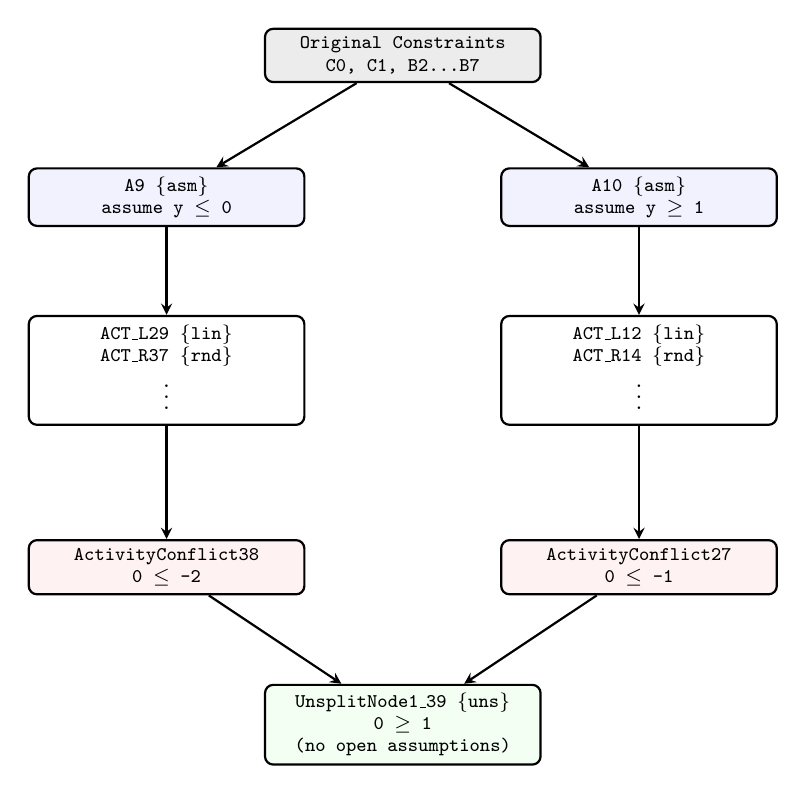
\begin{tikzpicture}[
  >=stealth,
  thick,
  node distance=1.5cm,
  base/.style={draw, rectangle, rounded corners=3pt, align=center, font=\scriptsize\ttfamily, minimum width=3.5cm, inner sep=3pt},
  root/.style={base, fill=gray!15},
  asm/.style={base, fill=blue!5},
  deriv/.style={base, fill=white},
  conflict/.style={base, fill=red!5},
  uns/.style={base, fill=green!5}
]

% 1. Root Node
\node[root] (root) at (0, 0) {Original Constraints\\C0, C1, B2...B7};

% 2. Assumptions (The Split)
\node[asm] (a9) at (-3, -1.8) {A9 \{asm\}\\assume y $\le$ 0};
\node[asm] (a10) at (3, -1.8) {A10 \{asm\}\\assume y $\ge$ 1};

% 3. Derivation Chains (lin and rnd)
\node[deriv] (leftchain) at (-3, -4) {\begin{tabular}{c} ACT\_L29 \{lin\} \\ ACT\_R37 \{rnd\} \\ $\vdots$ \end{tabular}};
\node[deriv] (rightchain) at (3, -4) {\begin{tabular}{c} ACT\_L12 \{lin\} \\ ACT\_R14 \{rnd\} \\ $\vdots$ \end{tabular}};

% 4. Absurdities (Branch Infeasible)
\node[conflict] (conf38) at (-3, -6.5) {ActivityConflict38\\0 $\le$ -2};
\node[conflict] (conf27) at (3, -6.5) {ActivityConflict27\\0 $\le$ -1};

% 5. The Unsplit (Merging the branches)
\node[uns] (uns) at (0, -8.5) {UnsplitNode1\_39 \{uns\}\\0 $\ge$ 1\\(no open assumptions)};

% Edges
\draw[->] (root) -- (a9);
\draw[->] (root) -- (a10);
\draw[->] (a9) -- (leftchain);
\draw[->] (a10) -- (rightchain);
\draw[->] (leftchain) -- (conf38);
\draw[->] (rightchain) -- (conf27);
\draw[->] (conf27) -- (uns);
\draw[->] (conf38) -- (uns);
\end{tikzpicture}
}
\end{minipage}
\caption{The real exact-\scip{} certificate (left, truncated) alongside its branch-and-bound derivation DAG (right, demonstration only) for the infeasible problem in~\autoref{eq:feas}.
The tree splits on integer variable $y$, tightening relaxations via \code{lin} and \code{rnd} steps until each branch reaches an absurdity.
The \code{uns} step merges the branches and discharges the assumptions.}
\label{fig:feas_combined}
\end{figure}

We next trace how \tool{} replays this flat certificate and verifies the branch argument in four steps.

\paragraph{Translate the certificate.}
\tool{} processes the flat derivation list shown in~\autoref{fig:feas_combined}.
Function \code{derToSStep} converts each parsed \code{DER} record into an \code{SStep}, consisting of a sensed row \code{SLe} and a reason \code{SReason}, such as \code{asm}, \code{lin}, \code{rnd}, or \code{uns}.
Function \code{initialPool} initializes the array-backed \code{CheckerPool} with the eight original \code{CON} rows converted by \code{conToSLe}.

\paragraph{Track branch assumptions.}
Each \code{CheckerEntry} contains a row and the finite set \code{SAsm} of assumptions on which it depends.
Rows \code{A9} and \code{A10} introduce the complementary cases $y\le0$ and $y\ge1$.
Function \code{entryOf} records an \code{asm} step's own bound and uses \code{collectReferencedAsms} so that \code{lin} and \code{rnd} steps inherit the assumptions of the rows they reference.

\paragraph{Check the branch derivations.}
For example, \code{ACT\_L12} cites the exact combination
\[
 -1\cdot C_0 + 10\cdot\code{A10} + 6\cdot B_4.
\]
\code{resolveRefs} retrieves rows 0, 10, and 4, and \code{checkLin} verifies that the signed multipliers are suitable for their senses, computes the sparse rational combination, and checks that it dominates the stated row.
The theorem \code{stepValidB\_sound} turns a successful Boolean step check into the declarative relation \code{Vipr.StepValid}; \code{Vipr.replay\_sound} then proves that the replayed entries are semantically sound over real assignments.
A \code{rnd} step is checked by \code{checkRnd}, which additionally uses \code{formIntB} to establish that the combined form is integer-valued before rounding its bound.
Repeating these checks derives \code{ActivityConflict27}, $0\le-1$, under \code{A10}, and \code{ActivityConflict38}, $0\le-2$, under \code{A9}.

\paragraph{Discharge the split and certify infeasibility.}
For the final reason \code{uns 27 10 38 9}, \code{stepValidB} uses \code{domSLe} to check that rows 27 and 38 each dominate the stated conclusion and \code{unsBoundsB} to check that rows 10 and 9 are complementary integer bounds.
Function \code{entryOf} then removes those branch bounds from the corresponding assumption sets.
The resulting row $0\ge1$ is absurd and has no open assumptions.
The production checker therefore returns \code{checkVipr cert = true}.
Its main theorem, \code{checkVipr\_sound}, yields \code{Vipr.ClaimValid cert}; because this certificate has \code{RTP infeas}, this states that no real assignment satisfying the declared integrality conditions can satisfy all constraints in~\autoref{eq:feas}.

%===============================================================================
\section{The \tool{} Approach}\label{sec:algorithm}


\begin{figure}[t]
  \centering
  \resizebox{\linewidth}{!}{%
  \begin{tikzpicture}[
    font=\sffamily,
    box/.style={
      draw=black, line width=0.95pt, rounded corners=1.2mm,
      minimum width=21mm, minimum height=22mm, align=center, inner sep=1.4mm
    },
    banner/.style={
      draw=black, line width=0.7pt, fill=#1, rounded corners=0.8mm,
      font=\scriptsize\bfseries, inner xsep=2mm, inner ysep=1.1mm
    },
    pill/.style={
      draw=black, line width=0.55pt, fill=white, rounded corners=0.7mm,
      font=\scriptsize, inner xsep=1.7mm, inner ysep=0.6mm
    },
    flow/.style={-{Stealth[length=2.4mm,width=1.9mm]}, line width=1pt,
      draw=blue!65!black, shorten <=2mm, shorten >=2mm},
    optional/.style={-{Stealth[length=2mm,width=1.5mm]}, dashed,
      line width=0.75pt, draw=orange!80!black,
      shorten <=1mm, shorten >=1mm}
  ]
    \node[box, fill=blue!16] (vipr) {%
      \textcolor{blue!70!black}{\fontsize{20}{22}\selectfont\faFile}\\[1.2mm]
      {\tiny\ttfamily VAR CON SOL DER}};
    \node[banner=blue!22] (viprB) at (vipr.north) {\vipr{}};

    \node[box, fill=orange!16, right=14mm of vipr] (parser) {%
      \textcolor{orange!80!black}{\fontsize{20}{22}\selectfont\faCode}\\[1.2mm]
      {\scriptsize\ttfamily parseVipr}};
    \node[banner=orange!22] (parserB) at (parser.north) {Frontend};

    \node[box, fill=white, right=14mm of parser] (ast) {%
      \textcolor{yellow!45!black}{\fontsize{20}{22}\selectfont\faSitemap}\\[1.2mm]
      {\scriptsize\ttfamily Vipr}};
    \node[banner=yellow!35] (astB) at (ast.north) {AST};

    \node[box, fill=red!11, minimum width=29mm, right=18mm of ast] (checker) {%
      \textcolor{red!65!black}{\fontsize{20}{22}\selectfont\faCogs}\\[0.8mm]
      {\scriptsize\ttfamily checkVipr}};
    \node[banner=red!16] (checkerB) at (checker.north) {Check};

    \node[box, fill=white, minimum width=38mm, right=21mm of checker] (proof) {%
      
\includegraphics[width=17mm]{figures/lean-logo}\\[0.8mm]
      {\tiny\ttfamily checkVipr\_sound}\\[-0.2mm]
      {\tiny\ttfamily checkViprInfeasibleSubset\_sound}};
    \node[banner=black!8] (proofB) at (proof.north) {Prove};

    \node[box, fill=green!14, minimum width=26mm, right=19mm of proof] (result) {%
      \textcolor{green!50!black}{\fontsize{20}{22}\selectfont\faCheckCircle}\\[0.8mm]
      {\scriptsize\ttfamily Vipr.ClaimValid}\\[-0.2mm]
      {\tiny infeasibility / range}};
    \node[banner=green!22] (resultB) at (result.north) {Result};

    \coordinate (sliceAnchor) at ($(ast)!0.5!(checker)$);
    \node[box, fill=orange!10, minimum width=21mm, minimum height=18mm,
      above=20mm of sliceAnchor] (slice) {%
      \textcolor{orange!80!black}{\fontsize{15}{17}\selectfont\faFilter}\\[0.6mm]
      {\scriptsize\ttfamily sliceVipr}\\[-0.2mm]
      {\tiny infeasibility only}};
    \node[banner=orange!18] (sliceB) at (slice.north) {Slice};

    \draw[flow] (vipr) -- node[pill, above=3mm] {text} (parser);
    \draw[flow] (parser) -- node[pill, above=3mm] {parse} (ast);
    \draw[flow] (ast) -- node[pill, above=3mm] {full replay} (checker);
    \draw[flow] (checker) -- node[pill, above=3mm]
      {returns \texttt{true}} (proof);
    \draw[flow] (proof) -- node[pill, above=3mm] {sound} (result);

    \draw[optional] (ast.north) |- (slice.west);
    \draw[optional] (slice.east) -| (checker.north);

    \node[fit=(parserB)(parser), dashed, draw=orange!70!black, line width=0.8pt,
      rounded corners=1.4mm, fill=none, inner xsep=3.2mm,
      inner ysep=3.4mm] (front) {};
    \node[fit=(astB)(ast)(checker)(proof)(result)(resultB),
      dashed, draw=black!70, line width=0.85pt, rounded corners=1.8mm,
      fill=none, inner xsep=4mm, inner ysep=4mm] (verified) {};
    \node[banner=orange!18] at (front.south) {trust boundary};
    \node[banner=yellow!40] at (verified.south)
      {formally verified core};

  \end{tikzpicture}%
  }
  \caption{\tool{}'s executable checker and soundness chain. The blue path
  replays the complete certificate. The dashed orange path is optional
  untrusted backward slicing for infeasibility certificates; checked subset
  conditions transport its result to the original MIP.}
  \label{fig:pipeline}
\end{figure}

\autoref{fig:pipeline} separates three parts of \tool{}: the textual frontend,
the executable checker, and the proof that Boolean acceptance implies the
claimed MIP result. The main soundness theorem begins with a parsed
\code{Vipr} value; correctness of \code{parseVipr} with respect to source text
is therefore a separate frontend concern.

\paragraph{Certificate Semantics}

A sparse linear form is represented as a list of variable-index and rational-coefficient pairs.
An \code{SLe} row pairs such a form and a rational right-hand side with a
sense: \code{L} for $\leq$, \code{G} for $\geq$, or \code{E} for equality.
The function \code{conSLes} converts the original \code{CON} records into sensed rows, while \code{viprSteps} applies \code{derToSStep} to every \code{DER} record.

This translation preserves the certificate's shared index space, so each derivation can resolve its references directly against the replay pool.
Although the representation uses exact rationals, its soundness is stated for real valuations whose declared integer variables have integer values.

\paragraph{Executable Replay}

The production checker stores replay entries in an array \code{CheckerPool}.
Each entry is a pair $(c,A)$ consisting of a row $c$ and the finite set $A$ of
branch assumptions on which it depends. The original constraints initialize
the array with empty assumption sets.

\begin{algorithm}[t]
\DontPrintSemicolon
\caption{Production checker \code{checkVipr}.}
\label{alg:checksem}
\KwIn{Parsed certificate $v$}
\If{$\neg\,\text{\code{solSectionB}}(v)$}{
  \KwRet{\code{false}}\tcp*[r]{Reject invalid solution data}
}
$P \gets \text{\code{initialPool}}(v)$\tcp*[r]{Array of original rows}
\ForEach{$s\in\text{\code{viprSteps}}(v)$}{
  \If{$\neg\,\text{\code{stepValidB}}(v,P,s)$}{
    \KwRet{\code{false}}\tcp*[r]{Reject the first invalid step}
  }
  $P.\text{\code{push}}(\text{\code{entryOf}}(P,s))$\tcp*[r]{Append row and assumptions}
}
\KwRet{$\text{\code{finalValidB}}(v,P.\text{\code{back?}})$}
\end{algorithm}

\autoref{alg:checksem} mirrors the implementation. The Boolean
\code{stepValidB} checks that all references point backward and validates the
selected \code{asm}, \code{lin}, \code{rnd}, \code{uns}, or \code{sol} rule.
Validation and replay are fused: after a successful check, \code{entryOf}
computes the new assumption set and appends the entry to the array.
Because \code{replaySteps?} recurses structurally over the finite step list,
the checker is total and terminating.

The final condition depends on \code{RTP}. For \code{infeas},
\code{finalValidB} requires an assumption-free absurd row. For a minimization
range, the derivation supplies the lower bound while a checked feasible
\code{SOL} witness supplies the upper bound; maximization reverses these roles.
Thus range acceptance checks both proof replay and the listed primal
solutions, rather than treating the absence of a contradiction as evidence of
feasibility.

\paragraph{Declarative Proof System and Soundness}

The semantic proof system is deliberately separate from the executable array
implementation. \code{Vipr.StepValid} specifies the mathematical validity of
one rule, \code{Vipr.DerivationValid} lifts it to a derivation, and
\code{Vipr.ProofValid} combines replay validity, solution validity, and
the appropriate final-row condition.
For example, a \code{lin} step is valid when every reference points to an
earlier entry and a sign-compatible exact rational combination of the
referenced rows dominates the stated row; replay assigns the new entry the
union of their open assumptions.

The theorem \code{stepValidB\_sound} maps successful Boolean checking of one
array-backed step to \code{Vipr.StepValid}. The replay refinement theorem
\code{replaySteps\_refines} lifts this correspondence to the complete
array replay, after which
\code{checkVipr\_refines} establishes
\code{Vipr.ProofValid}. Independently,
\code{Vipr.proofSystem\_sound} proves the soundness of the declarative
\vipr{} system. Their composition is the main implementation theorem:
\[
  \code{checkVipr v = true}
  \quad\Longrightarrow\quad
  \code{Vipr.ClaimValid v}.
\]
This is the statement of \code{checkVipr\_sound}. For
\code{RTP infeas}, \code{Vipr.ClaimValid} excludes every real feasible
assignment satisfying the integrality declarations. For \code{RTP range}, it
states that the listed solutions are valid and that every optimal objective
value lies in the reported interval.

\paragraph{Backward Slicing}

For infeasibility certificates, \code{sliceVipr} follows references backward
from the final contradiction, retains only reachable \code{CON} and
\code{DER} rows, and remaps their indices. The slicing code is an untrusted
optimization. The theorem \code{checkViprInfeasibleSubset\_sound} transports
infeasibility only when the concrete slice has the same integer variables,
every retained original row occurs in the original system, and
\code{checkVipr} accepts the slice. A generated reconstruction artifact
checks these premises for the particular certificate. Consequently, an
incorrect slice is rejected rather than changing the soundness claim. Range
certificates currently use complete replay because their solution witnesses
and objective bounds refer to the original problem.

\paragraph{Evaluation}

We evaluate the native \tool{} executable on 26 exact-\scip{} certificates:
20 infeasibility certificates from the ALU suite used in exact-MIP
experiments~\citep{eifler2023computational} and six objective-range
certificates from ALU and MIPLIB~3.0. \autoref{tab:evaluation} reports native
execution on an Apple M3 Pro. On the same 20 infeasibility certificates,
slicing reduces replay from 124,382 to 33,568 steps---a 73\% reduction---and
aggregate wall time from 8.49 to 3.44 seconds, a 2.5$\times$ speedup. All 46
measured invocations pass: complete and sliced replay for each infeasibility
certificate, and complete replay for each range certificate. Soundness follows
from the theorems above rather than from the execution environment.

\begin{center}
\begin{minipage}{0.94\linewidth}
\centering
\refstepcounter{table}
\label{tab:evaluation}
\small
\textbf{\tablename~\thetable:} Native \tool{} replay. The full and sliced
infeasibility rows use the same 20 certificates.
\par\smallskip
\setlength{\tabcolsep}{7pt}
\begin{tabular}{lrrr}
\toprule
Certificate mode & Certificates & Replayed steps & Wall time (s) \\
\midrule
Infeasibility, full   & 20 & 124,382 & 8.49 \\
Infeasibility, sliced & 20 &  33,568 & 3.44 \\
Objective range, full &  6 &  95,145 & 28.41 \\
\bottomrule
\end{tabular}
\end{minipage}
\end{center}

\paragraph{Trust Base}

At the theorem level, the trusted base is the standard \lean{} kernel, and the
development introduces no additional axioms. For a particular source file,
native execution additionally trusts the \vipr{} parser and the \lean{}
compiler and runtime. This is a common performance--trust tradeoff for verified
decision procedures using native evaluation, including \textsc{LratCatcher}
and \textsc{Pblean}%
~\citep{szeider2026lrat,szeider2026pblean}.

We also experimented with proof artifacts whose concrete Boolean equality is
discharged by kernel reduction using \code{decide +kernel}, removing the
\lean{} compiler and runtime from the trusted base. This mode did not complete
the full suite under a five-minute per-instance limit, so scalable kernel-only
replay remains future work.

%===============================================================================
\section{Related Work}\label{sec:related}
\paragraph{MIP certificate checking.}

\citet{cheung2017verifying} introduced \vipr{}, certificate support in exact \scip{}, and the C\texttt{++} checker \textsc{ViprChk}.
Closest to our work, \citet{wood2025satisfiability} formalize \vipr{} validity in \textsc{Why3}~\citep{filliatre2013why3} and relate it to a ground linear integer-real arithmetic formula, while a separate C\texttt{++} frontend emits SMT-LIB for \textsc{Cvc5}~\citep{barrett2010smt,barbosa2022cvc5}.
We instead implement certificate replay and prove the checker sound directly in
\lean{}, without relying on an external SMT solver in the soundness argument.

\paragraph{Formally verified certificate checking.}
\textsc{LratCatcher} checks SAT refutations in \lean{} by reflection~\citep{szeider2026lrat}.
For pseudo-Boolean reasoning, \textsc{Pblean} reflectively checks \textsc{VeriPB} certificates in \lean{}~\citep{szeider2026pblean}, while \textsc{CakePB} obtains a verified standalone checker through \textsc{HOL4} and \textsc{CakeML}~\citep{gocht2024end}.
These systems provide formally verified checking for SAT and pseudo-Boolean
proof systems. \tool{} extends this line of work to certificates produced by a
general MIP solver, including exact rational constraints, continuous and
integer variables, integrality-based rounding, and explicit discharge of branch
assumptions.

%===============================================================================
\section{Conclusion and Future Work}\label{sec:conclusion}

We presented \tool{}, a formally verified \lean{} checker for \vipr{}
infeasibility and objective-range certificates.
\tool{} checks linear combination, rounding, assumptions, and unsplitting, and proves that these checks preserve validity.
Its executable Boolean checker is linked by a \lean{} theorem to the claimed MIP
result, without relying on the solver, the reference checker, or an external
SMT solver for the soundness argument.

Future work will investigate completeness of the \vipr{} proof system,
formalize the checker's algorithmic complexity, verify the \vipr{} parser to
remove it from the trusted base, and scale kernel-only replay and evaluation to
larger certificates.

\paragraph{AI assistance disclosure.}
An LLM-based coding assistant was used during development to assist with
\lean{} implementation and proof engineering, benchmark scripting, and
manuscript editing. The assistant is not part of \tool{} or its trusted base.
All resulting code and proofs were reviewed by the authors, the formal
development was checked by \lean{}, and the authors take responsibility for
the paper and artifact.

\bibliographystyle{plainnat}
\bibliography{main}

%%%%%%%%%%%%%%%%%%%%%%%%%%%%%%%%%%%%%%%%%%%%%%%%%%%%%%%%%%%%

\newpage
% \section*{NeurIPS Paper Checklist}

%%% BEGIN INSTRUCTIONS %%%
The checklist is designed to encourage best practices for responsible machine learning research, addressing issues of reproducibility, transparency, research ethics, and societal impact. Do not remove the checklist: {\bf The papers not including the checklist will be desk rejected.} The checklist should follow the references and follow the (optional) supplemental material.  The checklist does NOT count towards the page
limit. 

Please read the checklist guidelines carefully for information on how to answer these questions. For each question in the checklist:
\begin{itemize}
    \item You should answer \answerYes{}, \answerNo{}, or \answerNA{}.
    \item \answerNA{} means either that the question is Not Applicable for that particular paper or the relevant information is Not Available.
    \item Please provide a short (1--2 sentence) justification right after your answer (even for \answerNA). 
   % \item {\bf The papers not including the checklist will be desk rejected.}
\end{itemize}

{\bf The checklist answers are an integral part of your paper submission.} They are visible to the reviewers, area chairs, senior area chairs, and ethics reviewers. You will also be asked to include it (after eventual revisions) with the final version of your paper, and its final version will be published with the paper.

The reviewers of your paper will be asked to use the checklist as one of the factors in their evaluation. While \answerYes{} is generally preferable to \answerNo{}, it is perfectly acceptable to answer \answerNo{} provided a proper justification is given (e.g., error bars are not reported because it would be too computationally expensive'' or ``we were unable to find the license for the dataset we used''). In general, answering \answerNo{} or \answerNA{} is not grounds for rejection. While the questions are phrased in a binary way, we acknowledge that the true answer is often more nuanced, so please just use your best judgment and write a justification to elaborate. All supporting evidence can appear either in the main paper or the supplemental material, provided in appendix. If you answer \answerYes{} to a question, in the justification please point to the section(s) where related material for the question can be found.

IMPORTANT, please:
\begin{itemize}
    \item {\bf Delete this instruction block, but keep the section heading ``NeurIPS Paper Checklist"},
    \item  {\bf Keep the checklist subsection headings, questions/answers and guidelines below.}
    \item {\bf Do not modify the questions and only use the provided macros for your answers}.
\end{itemize} 
 

%%% END INSTRUCTIONS %%%


\begin{enumerate}

\item {\bf Claims}
    \item[] Question: Do the main claims made in the abstract and introduction accurately reflect the paper's contributions and scope?
    \item[] Answer: \answerTODO{} % Replace by \answerYes{}, \answerNo{}, or \answerNA{}.
    \item[] Justification: \justificationTODO{}
    \item[] Guidelines:
    \begin{itemize}
        \item The answer \answerNA{} means that the abstract and introduction do not include the claims made in the paper.
        \item The abstract and/or introduction should clearly state the claims made, including the contributions made in the paper and important assumptions and limitations. A \answerNo{} or \answerNA{} answer to this question will not be perceived well by the reviewers. 
        \item The claims made should match theoretical and experimental results, and reflect how much the results can be expected to generalize to other settings. 
        \item It is fine to include aspirational goals as motivation as long as it is clear that these goals are not attained by the paper. 
    \end{itemize}

\item {\bf Limitations}
    \item[] Question: Does the paper discuss the limitations of the work performed by the authors?
    \item[] Answer: \answerTODO{} % Replace by \answerYes{}, \answerNo{}, or \answerNA{}.
    \item[] Justification: \justificationTODO{}
    \item[] Guidelines:
    \begin{itemize}
        \item The answer \answerNA{} means that the paper has no limitation while the answer \answerNo{} means that the paper has limitations, but those are not discussed in the paper. 
        \item The authors are encouraged to create a separate ``Limitations'' section in their paper.
        \item The paper should point out any strong assumptions and how robust the results are to violations of these assumptions (e.g., independence assumptions, noiseless settings, model well-specification, asymptotic approximations only holding locally). The authors should reflect on how these assumptions might be violated in practice and what the implications would be.
        \item The authors should reflect on the scope of the claims made, e.g., if the approach was only tested on a few datasets or with a few runs. In general, empirical results often depend on implicit assumptions, which should be articulated.
        \item The authors should reflect on the factors that influence the performance of the approach. For example, a facial recognition algorithm may perform poorly when image resolution is low or images are taken in low lighting. Or a speech-to-text system might not be used reliably to provide closed captions for online lectures because it fails to handle technical jargon.
        \item The authors should discuss the computational efficiency of the proposed algorithms and how they scale with dataset size.
        \item If applicable, the authors should discuss possible limitations of their approach to address problems of privacy and fairness.
        \item While the authors might fear that complete honesty about limitations might be used by reviewers as grounds for rejection, a worse outcome might be that reviewers discover limitations that aren't acknowledged in the paper. The authors should use their best judgment and recognize that individual actions in favor of transparency play an important role in developing norms that preserve the integrity of the community. Reviewers will be specifically instructed to not penalize honesty concerning limitations.
    \end{itemize}

\item {\bf Theory assumptions and proofs}
    \item[] Question: For each theoretical result, does the paper provide the full set of assumptions and a complete (and correct) proof?
    \item[] Answer: \answerTODO{} % Replace by \answerYes{}, \answerNo{}, or \answerNA{}.
    \item[] Justification: \justificationTODO{}
    \item[] Guidelines:
    \begin{itemize}
        \item The answer \answerNA{} means that the paper does not include theoretical results. 
        \item All the theorems, formulas, and proofs in the paper should be numbered and cross-referenced.
        \item All assumptions should be clearly stated or referenced in the statement of any theorems.
        \item The proofs can either appear in the main paper or the supplemental material, but if they appear in the supplemental material, the authors are encouraged to provide a short proof sketch to provide intuition. 
        \item Inversely, any informal proof provided in the core of the paper should be complemented by formal proofs provided in appendix or supplemental material.
        \item Theorems and Lemmas that the proof relies upon should be properly referenced. 
    \end{itemize}

    \item {\bf Experimental result reproducibility}
    \item[] Question: Does the paper fully disclose all the information needed to reproduce the main experimental results of the paper to the extent that it affects the main claims and/or conclusions of the paper (regardless of whether the code and data are provided or not)?
    \item[] Answer: \answerTODO{} % Replace by \answerYes{}, \answerNo{}, or \answerNA{}.
    \item[] Justification: \justificationTODO{}
    \item[] Guidelines:
    \begin{itemize}
        \item The answer \answerNA{} means that the paper does not include experiments.
        \item If the paper includes experiments, a \answerNo{} answer to this question will not be perceived well by the reviewers: Making the paper reproducible is important, regardless of whether the code and data are provided or not.
        \item If the contribution is a dataset and\slash or model, the authors should describe the steps taken to make their results reproducible or verifiable. 
        \item Depending on the contribution, reproducibility can be accomplished in various ways. For example, if the contribution is a novel architecture, describing the architecture fully might suffice, or if the contribution is a specific model and empirical evaluation, it may be necessary to either make it possible for others to replicate the model with the same dataset, or provide access to the model. In general. releasing code and data is often one good way to accomplish this, but reproducibility can also be provided via detailed instructions for how to replicate the results, access to a hosted model (e.g., in the case of a large language model), releasing of a model checkpoint, or other means that are appropriate to the research performed.
        \item While NeurIPS does not require releasing code, the conference does require all submissions to provide some reasonable avenue for reproducibility, which may depend on the nature of the contribution. For example
        \begin{enumerate}
            \item If the contribution is primarily a new algorithm, the paper should make it clear how to reproduce that algorithm.
            \item If the contribution is primarily a new model architecture, the paper should describe the architecture clearly and fully.
            \item If the contribution is a new model (e.g., a large language model), then there should either be a way to access this model for reproducing the results or a way to reproduce the model (e.g., with an open-source dataset or instructions for how to construct the dataset).
            \item We recognize that reproducibility may be tricky in some cases, in which case authors are welcome to describe the particular way they provide for reproducibility. In the case of closed-source models, it may be that access to the model is limited in some way (e.g., to registered users), but it should be possible for other researchers to have some path to reproducing or verifying the results.
        \end{enumerate}
    \end{itemize}


\item {\bf Open access to data and code}
    \item[] Question: Does the paper provide open access to the data and code, with sufficient instructions to faithfully reproduce the main experimental results, as described in supplemental material?
    \item[] Answer: \answerTODO{} % Replace by \answerYes{}, \answerNo{}, or \answerNA{}.
    \item[] Justification: \justificationTODO{}
    \item[] Guidelines:
    \begin{itemize}
        \item The answer \answerNA{} means that paper does not include experiments requiring code.
        \item Please see the NeurIPS code and data submission guidelines (\url{https://neurips.cc/public/guides/CodeSubmissionPolicy}) for more details.
        \item While we encourage the release of code and data, we understand that this might not be possible, so \answerNo{} is an acceptable answer. Papers cannot be rejected simply for not including code, unless this is central to the contribution (e.g., for a new open-source benchmark).
        \item The instructions should contain the exact command and environment needed to run to reproduce the results. See the NeurIPS code and data submission guidelines (\url{https://neurips.cc/public/guides/CodeSubmissionPolicy}) for more details.
        \item The authors should provide instructions on data access and preparation, including how to access the raw data, preprocessed data, intermediate data, and generated data, etc.
        \item The authors should provide scripts to reproduce all experimental results for the new proposed method and baselines. If only a subset of experiments are reproducible, they should state which ones are omitted from the script and why.
        \item At submission time, to preserve anonymity, the authors should release anonymized versions (if applicable).
        \item Providing as much information as possible in supplemental material (appended to the paper) is recommended, but including URLs to data and code is permitted.
    \end{itemize}


\item {\bf Experimental setting/details}
    \item[] Question: Does the paper specify all the training and test details (e.g., data splits, hyperparameters, how they were chosen, type of optimizer) necessary to understand the results?
    \item[] Answer: \answerTODO{} % Replace by \answerYes{}, \answerNo{}, or \answerNA{}.
    \item[] Justification: \justificationTODO{}
    \item[] Guidelines:
    \begin{itemize}
        \item The answer \answerNA{} means that the paper does not include experiments.
        \item The experimental setting should be presented in the core of the paper to a level of detail that is necessary to appreciate the results and make sense of them.
        \item The full details can be provided either with the code, in appendix, or as supplemental material.
    \end{itemize}

\item {\bf Experiment statistical significance}
    \item[] Question: Does the paper report error bars suitably and correctly defined or other appropriate information about the statistical significance of the experiments?
    \item[] Answer: \answerTODO{} % Replace by \answerYes{}, \answerNo{}, or \answerNA{}.
    \item[] Justification: \justificationTODO{}
    \item[] Guidelines:
    \begin{itemize}
        \item The answer \answerNA{} means that the paper does not include experiments.
        \item The authors should answer \answerYes{} if the results are accompanied by error bars, confidence intervals, or statistical significance tests, at least for the experiments that support the main claims of the paper.
        \item The factors of variability that the error bars are capturing should be clearly stated (for example, train/test split, initialization, random drawing of some parameter, or overall run with given experimental conditions).
        \item The method for calculating the error bars should be explained (closed form formula, call to a library function, bootstrap, etc.)
        \item The assumptions made should be given (e.g., Normally distributed errors).
        \item It should be clear whether the error bar is the standard deviation or the standard error of the mean.
        \item It is OK to report 1-sigma error bars, but one should state it. The authors should preferably report a 2-sigma error bar than state that they have a 96\% CI, if the hypothesis of Normality of errors is not verified.
        \item For asymmetric distributions, the authors should be careful not to show in tables or figures symmetric error bars that would yield results that are out of range (e.g., negative error rates).
        \item If error bars are reported in tables or plots, the authors should explain in the text how they were calculated and reference the corresponding figures or tables in the text.
    \end{itemize}

\item {\bf Experiments compute resources}
    \item[] Question: For each experiment, does the paper provide sufficient information on the computer resources (type of compute workers, memory, time of execution) needed to reproduce the experiments?
    \item[] Answer: \answerTODO{} % Replace by \answerYes{}, \answerNo{}, or \answerNA{}.
    \item[] Justification: \justificationTODO{}
    \item[] Guidelines:
    \begin{itemize}
        \item The answer \answerNA{} means that the paper does not include experiments.
        \item The paper should indicate the type of compute workers CPU or GPU, internal cluster, or cloud provider, including relevant memory and storage.
        \item The paper should provide the amount of compute required for each of the individual experimental runs as well as estimate the total compute. 
        \item The paper should disclose whether the full research project required more compute than the experiments reported in the paper (e.g., preliminary or failed experiments that didn't make it into the paper). 
    \end{itemize}
    
\item {\bf Code of ethics}
    \item[] Question: Does the research conducted in the paper conform, in every respect, with the NeurIPS Code of Ethics \url{https://neurips.cc/public/EthicsGuidelines}?
    \item[] Answer: \answerTODO{} % Replace by \answerYes{}, \answerNo{}, or \answerNA{}.
    \item[] Justification: \justificationTODO{}
    \item[] Guidelines:
    \begin{itemize}
        \item The answer \answerNA{} means that the authors have not reviewed the NeurIPS Code of Ethics.
        \item If the authors answer \answerNo, they should explain the special circumstances that require a deviation from the Code of Ethics.
        \item The authors should make sure to preserve anonymity (e.g., if there is a special consideration due to laws or regulations in their jurisdiction).
    \end{itemize}


\item {\bf Broader impacts}
    \item[] Question: Does the paper discuss both potential positive societal impacts and negative societal impacts of the work performed?
    \item[] Answer: \answerTODO{} % Replace by \answerYes{}, \answerNo{}, or \answerNA{}.
    \item[] Justification: \justificationTODO{}
    \item[] Guidelines:
    \begin{itemize}
        \item The answer \answerNA{} means that there is no societal impact of the work performed.
        \item If the authors answer \answerNA{} or \answerNo, they should explain why their work has no societal impact or why the paper does not address societal impact.
        \item Examples of negative societal impacts include potential malicious or unintended uses (e.g., disinformation, generating fake profiles, surveillance), fairness considerations (e.g., deployment of technologies that could make decisions that unfairly impact specific groups), privacy considerations, and security considerations.
        \item The conference expects that many papers will be foundational research and not tied to particular applications, let alone deployments. However, if there is a direct path to any negative applications, the authors should point it out. For example, it is legitimate to point out that an improvement in the quality of generative models could be used to generate Deepfakes for disinformation. On the other hand, it is not needed to point out that a generic algorithm for optimizing neural networks could enable people to train models that generate Deepfakes faster.
        \item The authors should consider possible harms that could arise when the technology is being used as intended and functioning correctly, harms that could arise when the technology is being used as intended but gives incorrect results, and harms following from (intentional or unintentional) misuse of the technology.
        \item If there are negative societal impacts, the authors could also discuss possible mitigation strategies (e.g., gated release of models, providing defenses in addition to attacks, mechanisms for monitoring misuse, mechanisms to monitor how a system learns from feedback over time, improving the efficiency and accessibility of ML).
    \end{itemize}
    
\item {\bf Safeguards}
    \item[] Question: Does the paper describe safeguards that have been put in place for responsible release of data or models that have a high risk for misuse (e.g., pre-trained language models, image generators, or scraped datasets)?
    \item[] Answer: \answerTODO{} % Replace by \answerYes{}, \answerNo{}, or \answerNA{}.
    \item[] Justification: \justificationTODO{}
    \item[] Guidelines:
    \begin{itemize}
        \item The answer \answerNA{} means that the paper poses no such risks.
        \item Released models that have a high risk for misuse or dual-use should be released with necessary safeguards to allow for controlled use of the model, for example by requiring that users adhere to usage guidelines or restrictions to access the model or implementing safety filters. 
        \item Datasets that have been scraped from the Internet could pose safety risks. The authors should describe how they avoided releasing unsafe images.
        \item We recognize that providing effective safeguards is challenging, and many papers do not require this, but we encourage authors to take this into account and make a best faith effort.
    \end{itemize}

\item {\bf Licenses for existing assets}
    \item[] Question: Are the creators or original owners of assets (e.g., code, data, models), used in the paper, properly credited and are the license and terms of use explicitly mentioned and properly respected?
    \item[] Answer: \answerTODO{} % Replace by \answerYes{}, \answerNo{}, or \answerNA{}.
    \item[] Justification: \justificationTODO{}
    \item[] Guidelines:
    \begin{itemize}
        \item The answer \answerNA{} means that the paper does not use existing assets.
        \item The authors should cite the original paper that produced the code package or dataset.
        \item The authors should state which version of the asset is used and, if possible, include a URL.
        \item The name of the license (e.g., CC-BY 4.0) should be included for each asset.
        \item For scraped data from a particular source (e.g., website), the copyright and terms of service of that source should be provided.
        \item If assets are released, the license, copyright information, and terms of use in the package should be provided. For popular datasets, \url{paperswithcode.com/datasets} has curated licenses for some datasets. Their licensing guide can help determine the license of a dataset.
        \item For existing datasets that are re-packaged, both the original license and the license of the derived asset (if it has changed) should be provided.
        \item If this information is not available online, the authors are encouraged to reach out to the asset's creators.
    \end{itemize}

\item {\bf New assets}
    \item[] Question: Are new assets introduced in the paper well documented and is the documentation provided alongside the assets?
    \item[] Answer: \answerTODO{} % Replace by \answerYes{}, \answerNo{}, or \answerNA{}.
    \item[] Justification: \justificationTODO{}
    \item[] Guidelines:
    \begin{itemize}
        \item The answer \answerNA{} means that the paper does not release new assets.
        \item Researchers should communicate the details of the dataset\slash code\slash model as part of their submissions via structured templates. This includes details about training, license, limitations, etc. 
        \item The paper should discuss whether and how consent was obtained from people whose asset is used.
        \item At submission time, remember to anonymize your assets (if applicable). You can either create an anonymized URL or include an anonymized zip file.
    \end{itemize}

\item {\bf Crowdsourcing and research with human subjects}
    \item[] Question: For crowdsourcing experiments and research with human subjects, does the paper include the full text of instructions given to participants and screenshots, if applicable, as well as details about compensation (if any)? 
    \item[] Answer: \answerTODO{} % Replace by \answerYes{}, \answerNo{}, or \answerNA{}.
    \item[] Justification: \justificationTODO{}
    \item[] Guidelines:
    \begin{itemize}
        \item The answer \answerNA{} means that the paper does not involve crowdsourcing nor research with human subjects.
        \item Including this information in the supplemental material is fine, but if the main contribution of the paper involves human subjects, then as much detail as possible should be included in the main paper. 
        \item According to the NeurIPS Code of Ethics, workers involved in data collection, curation, or other labor should be paid at least the minimum wage in the country of the data collector. 
    \end{itemize}

\item {\bf Institutional review board (IRB) approvals or equivalent for research with human subjects}
    \item[] Question: Does the paper describe potential risks incurred by study participants, whether such risks were disclosed to the subjects, and whether Institutional Review Board (IRB) approvals (or an equivalent approval/review based on the requirements of your country or institution) were obtained?
    \item[] Answer: \answerTODO{} % Replace by \answerYes{}, \answerNo{}, or \answerNA{}.
    \item[] Justification: \justificationTODO{}
    \item[] Guidelines:
    \begin{itemize}
        \item The answer \answerNA{} means that the paper does not involve crowdsourcing nor research with human subjects.
        \item Depending on the country in which research is conducted, IRB approval (or equivalent) may be required for any human subjects research. If you obtained IRB approval, you should clearly state this in the paper. 
        \item We recognize that the procedures for this may vary significantly between institutions and locations, and we expect authors to adhere to the NeurIPS Code of Ethics and the guidelines for their institution. 
        \item For initial submissions, do not include any information that would break anonymity (if applicable), such as the institution conducting the review.
    \end{itemize}

\item {\bf Declaration of LLM usage}
    \item[] Question: Does the paper describe the usage of LLMs if it is an important, original, or non-standard component of the core methods in this research? Note that if the LLM is used only for writing, editing, or formatting purposes and does \emph{not} impact the core methodology, scientific rigor, or originality of the research, declaration is not required.
    %this research? 
    \item[] Answer: \answerYes{}
    \item[] Justification: Section~\ref{sec:conclusion} discloses the use of an
    LLM-based coding assistant for \lean{} implementation and proof engineering,
    benchmark scripting, and manuscript editing, together with the authors'
    validation and responsibility for the resulting work.
    \item[] Guidelines:
    \begin{itemize}
        \item The answer \answerNA{} means that the core method development in this research does not involve LLMs as any important, original, or non-standard components.
        \item Please refer to our LLM policy in the NeurIPS handbook for what should or should not be described.
    \end{itemize}

\end{enumerate}



\end{document}
